
\chapter{Einleitung}

\section{Motivation}
Der Begriff \enquote{autonomes Fahren} hat spätestens seit den Tesla Autos einen allgemeinen Bekanntheitsgrad erreicht. Um ein Auto selbstständig fahren lassen zu können, müssen erst viele Hürden gemeistert werden, zum Beispiel das Spur halten, auch bei fehlenden Fahrspurmarkierungen, das Interpretieren von Stoppschildern und navigieren durch komplexen Kreuzungen. \todo{ref tesla.com?}

Bevor das Auto Entscheidungen treffen kann, muss es zuallererst ein Modell seines Umfelds erstellen oder zur Verfügung gestellt bekommen. Aber vielleicht kann ein Auto nicht immer selbständig genügend Informationen zu seinem Umfeld sammeln? \todo{(huhuhu Server implied huhuhu)}
%Diese Arbeit beschäftigt sich mit genau dem Thema, einem selbst fahrendem Auto Informationen zu anderen Teilnehmern an einer Kreuzung zu vermitteln.
\todo{fix 404}

\section{Projektkontext}
\begin{figure}[H]
	\label{test 123}
	\centering
	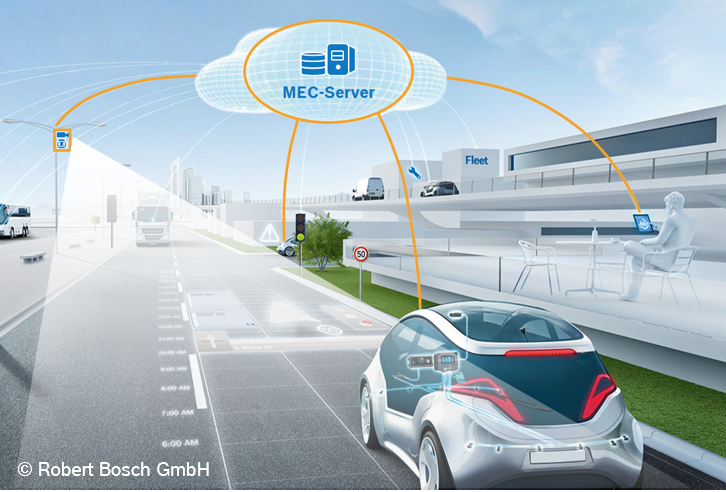
\includegraphics[width=\textwidth]{images/MECView_Schaubild_BoschStyle_V2.png}
	\caption{MEC-View Schaubild der Robert Bosch GmbH \cite{mec:home} {}}
	\captionsource{\url{https://www.uni-due.de/~hp0309/images/Schaubild_BoschStyle_V2.png}}
\end{figure}

\gls{mec:bmwi}
\todo{Forschungsprojekt MECView, BMWi oder so}

\section{Zielsetzung}

Das Ziel ist es, eine alternative Implementierung des MEC-View Servers in Rust zu schaffen.
Durch die Garantien \todo{ref} von Rust wird erhofft, dass der menschliche Faktor als Fehlerquelle gemindert wird und somit eine fehlertolerantere und sicherere Implementation geschaffen wird.
\todo{möglichst Beibehalt der Architektur?}


\section{Aufbau der Arbeit}

Diese Arbeit ist im wesentlichen in die folgenden Themengebiete aufgeteilt: Grundlagen, Anforderungs- und Systemanalyse, Systementwurf und Implementation und Auswertung.

Im Themengebiet Grundlagen sollen wesentliche Bestandteile dieser Arbeit erläutert und erklärt werden.
Hierzu zählt zum einen die Programmiersprache Rust in ihrer Entstehungsgeschichte \todo{ref}, Garantien \todo{ref}  und Sprachfeatures \todo{ref}, zum anderen die hochperformante, serverbasierte Kommunikationsplattform mit ihren Protokollen \todo{ref} und dem Systemkontext in dem diese betrieben wird.

In der Anforderungs- und Systemanalyse wird der Kontext in dem das System betrieben werden soll genauer betrachtet. Umzusetzende funktionale und nicht-funktionale Anforderungen werden aufgestellt sowie eine Übersicht von Systemen mit denen interagiert wird.

Das Themengebiet Systementwurf und Implementation befasst sich mit dem theoretischen und praktischen Lösen der im vorherigen Kapitel aufgestellten Anforderungen. Aufgrund der Tatsache, dass es sich hierbei
um eine alternative Implementation handelt, wird zur bestehenden C++ Implementation Bezug genommen.
Auf architektonische Unterschiede im Systementwurf, die sich aufgrund von Sprach- und Bibliotheksunterschiede, werden hier genauer beschrieben.

Zuletzt wird eine Auswertung der Implementation aufgezeigt. \todo{michael.write\_more();}